\scanpage{17}
\figure{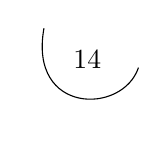
\begin{tikzpicture}[x=1cm,y=1cm]
\node at (0,0) {\mspage{14}};
\draw (-.55,.4) .. controls (-.75,-.7) and (.45,-.7) .. (.65,-.1);
\end{tikzpicture}}
\uline{Cor} Soit $\mathcal E$ un anneau gradué, \inserted{\figure{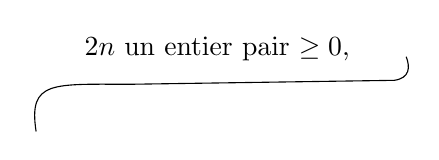
\begin{tikzpicture}[x=1cm,y=1cm]
\node at (0,.35) {$2n$ un entier pair $\geq0$,};
\draw (-2.3,-.7) .. controls (-2.4,-.05) and (-2.1,-.1) .. (-1.1,-.1) --(2.25,-.05) .. controls (2.45,-.02) and (2.45,.12) .. (2.4,.25);
\end{tikzpicture}}} et soit $L\in\mathcal E^{(2)}$.
S'il existe un hom d'anneaux gradués
\[
u:\Phi\longrightarrow\mathcal E
\]
tel que $u(\mathbf L)=L$, et tel que les $u(\boldsymbol\pi_i)=\pi_i$ définissent la graduation de $\mathcal E$ par $(1.3)$, alors un tel $u$ est uniquement déterminé, et les $\pi_i$ sont déterminés de façon unique, en termes de la structure \inserted{\uline{d'anneau}} graduée de $\mathcal E$ par les conditions $(1.1)$ et $(1.3)$.
\inserted{Si on se donne $\pi_i$ satisfaisant les conditions \deleted{\unsure{En l'absence des} $\pi_i$},}
\margin{\figure{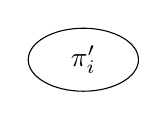
\begin{tikzpicture}\node at (0,0) {$\unsure{\pi'_i}$};\draw (0,0) ellipse (.7cm and .4cm);\end{tikzpicture}}}
l'existence de $u$ équivaut alors à \deleted{\unsure{l'existence}} la vérification, pour tt $0\leq i\leq n$, de la condition
\[
\text{``}\ \exists w_i\in\mathcal E^{-(2n-2i)}\text{ tel que}\quad(w_iL^{n-i}-1)\pi_{\deleted{\unsure{i}}\inserted{2n-i}}\deleted{=0}\text{''}=0,
\]
et \deleted{\unsure{alors}} le système des $\Lambda=u(\boldsymbol\Lambda)$, \deleted{et} $\pi_{i,\alpha}=u(\boldsymbol\pi_{i,\alpha})$ est alors caractérisé (en termes de $L$ et des $\pi_i$) par les équations $(6.14)$.
\margin{On a aussi : $\exists$ un module fidèle $M^*$ sous $\mathcal E^*$ tel que \unsure{par sa graduation} \unsure{coïncide avec} $\unsure{\pi_i}$ .... (\unsure{donc ceci pour tt i}). \deleted{\unsure{Si on dit}} \unsure{Tout précédent}.}
De la donnée des $\pi_i$, l'existence de $u$ équivaut à l'existence d'un module \uline{gradué} fidèle sous $\mathcal E^*$, \deleted{tel que} \unsure{$\mathcal E^*$} (\unsure{définie par les} $\pi_i\in\operatorname{End}(M^*)$), et tel que \figure{\begin{tikzpicture}[x=.35cm,y=.35cm,baseline]
\fill (0,0) ellipse (.09 and .045);
\fill (.5,.06) ellipse (.065 and .05);
\fill (.8,.07) ellipse (.07 and .045);
\fill (1.15,.12) ellipse (.09 and .04);
\fill (1.5,.15) ellipse (.055 and .05);
\draw[line width=.8pt] (1.9,.17) .. controls (2.05,.23) and (2.08,.23) .. (2.2,.18);
\draw[line width=.8pt] (2.5,.2)--(2.8,.21);
\fill (4.4,.22) circle (.13);
\end{tikzpicture}}

\uline{Question} Si on ne se donne \uline{pas} la graduation de $\mathcal E$ :
\inserted{\figure{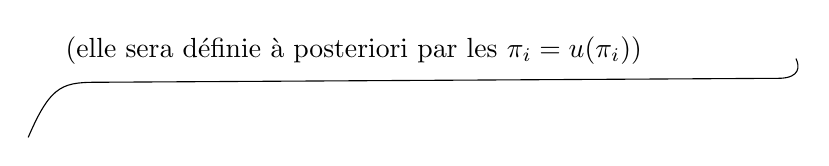
\begin{tikzpicture}[x=1cm,y=1cm]
\node[anchor=west] at (0,.35) {(elle sera définie à posteriori par les $\pi_i=u(\boldsymbol\pi_i)$)};
\draw (-.35,-.75) .. controls (-.05,-.05) and (.1,-.05) .. (.6,-.05) --(9.2,.0) .. controls (9.45,.01) and (9.45,.15) .. (9.4,.25);
\end{tikzpicture}}}
\unsure{pourrait-il|serait-il} vrai qu'il y a au plus un hom $\Phi\longrightarrow\mathcal E$ tel que $u(\mathbf L)=L$ !

\figure{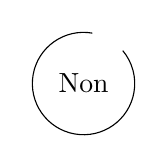
\begin{tikzpicture}\node at (0,0) {Non};\draw (80:.65cm) arc[start angle=80,end angle=400,radius=.65cm];\end{tikzpicture}}, déjà dans le cas $n=1$, $2n=2$, où il y a une base de $\Phi$ formée de $\pi_0,\pi_1,\pi_2,L,\Lambda$, et où $\mathbb Z[L]$ n'est que $\mathbb Z+\mathbb ZL$ ! Il faut donc se donner en même temps \uline{$L$ et les $\pi_i$}.
\mspage{16}
